% ============================================================
%  CAPÍTULO 2 — MARCO REFERENCIAL
% ============================================================
\chapter{Marco Referencial}

Este capítulo cubre dos temas. Primero, el estado del arte en detección
de \ac{MAP}: trabajos previos, métodos utilizados y sus limitaciones.
Segundo, la base teórica del trabajo: tipos de \ac{MAP} en Colombia,
imágenes multiespectrales, índices espectrales, calibración radiométrica,
alineación de bandas, selección de características y algoritmos de
clasificación.

% -------------------------------------------------------------
\section{Antecedentes}

En la literatura especializada se recogen numerosos estudios sobre la
detección de \ac{MAP} en los cuales se aplican métodos muy variados.
Tomando como referencia Scopus con las palabras clave
\textit{``landmine AND detection''}, en los últimos 30 años se observa
un interés sostenido de la comunidad científica, con un pico máximo entre
2004 y 2005 y una estabilización en torno a las 80 publicaciones anuales
en el período 2020--2025 (véase Figura~\ref{fig:tendencia_scopus}).
Estados Unidos encabeza el listado de países con mayor producción de
artículos, seguido por Japón y China. Para Colombia se registran 51
publicaciones, aunque en ninguna se identifica el uso de imágenes
multiespectrales como técnica de detección \cite{IsaacAnteproyecto}.

\begin{figure}[H]
  \centering
  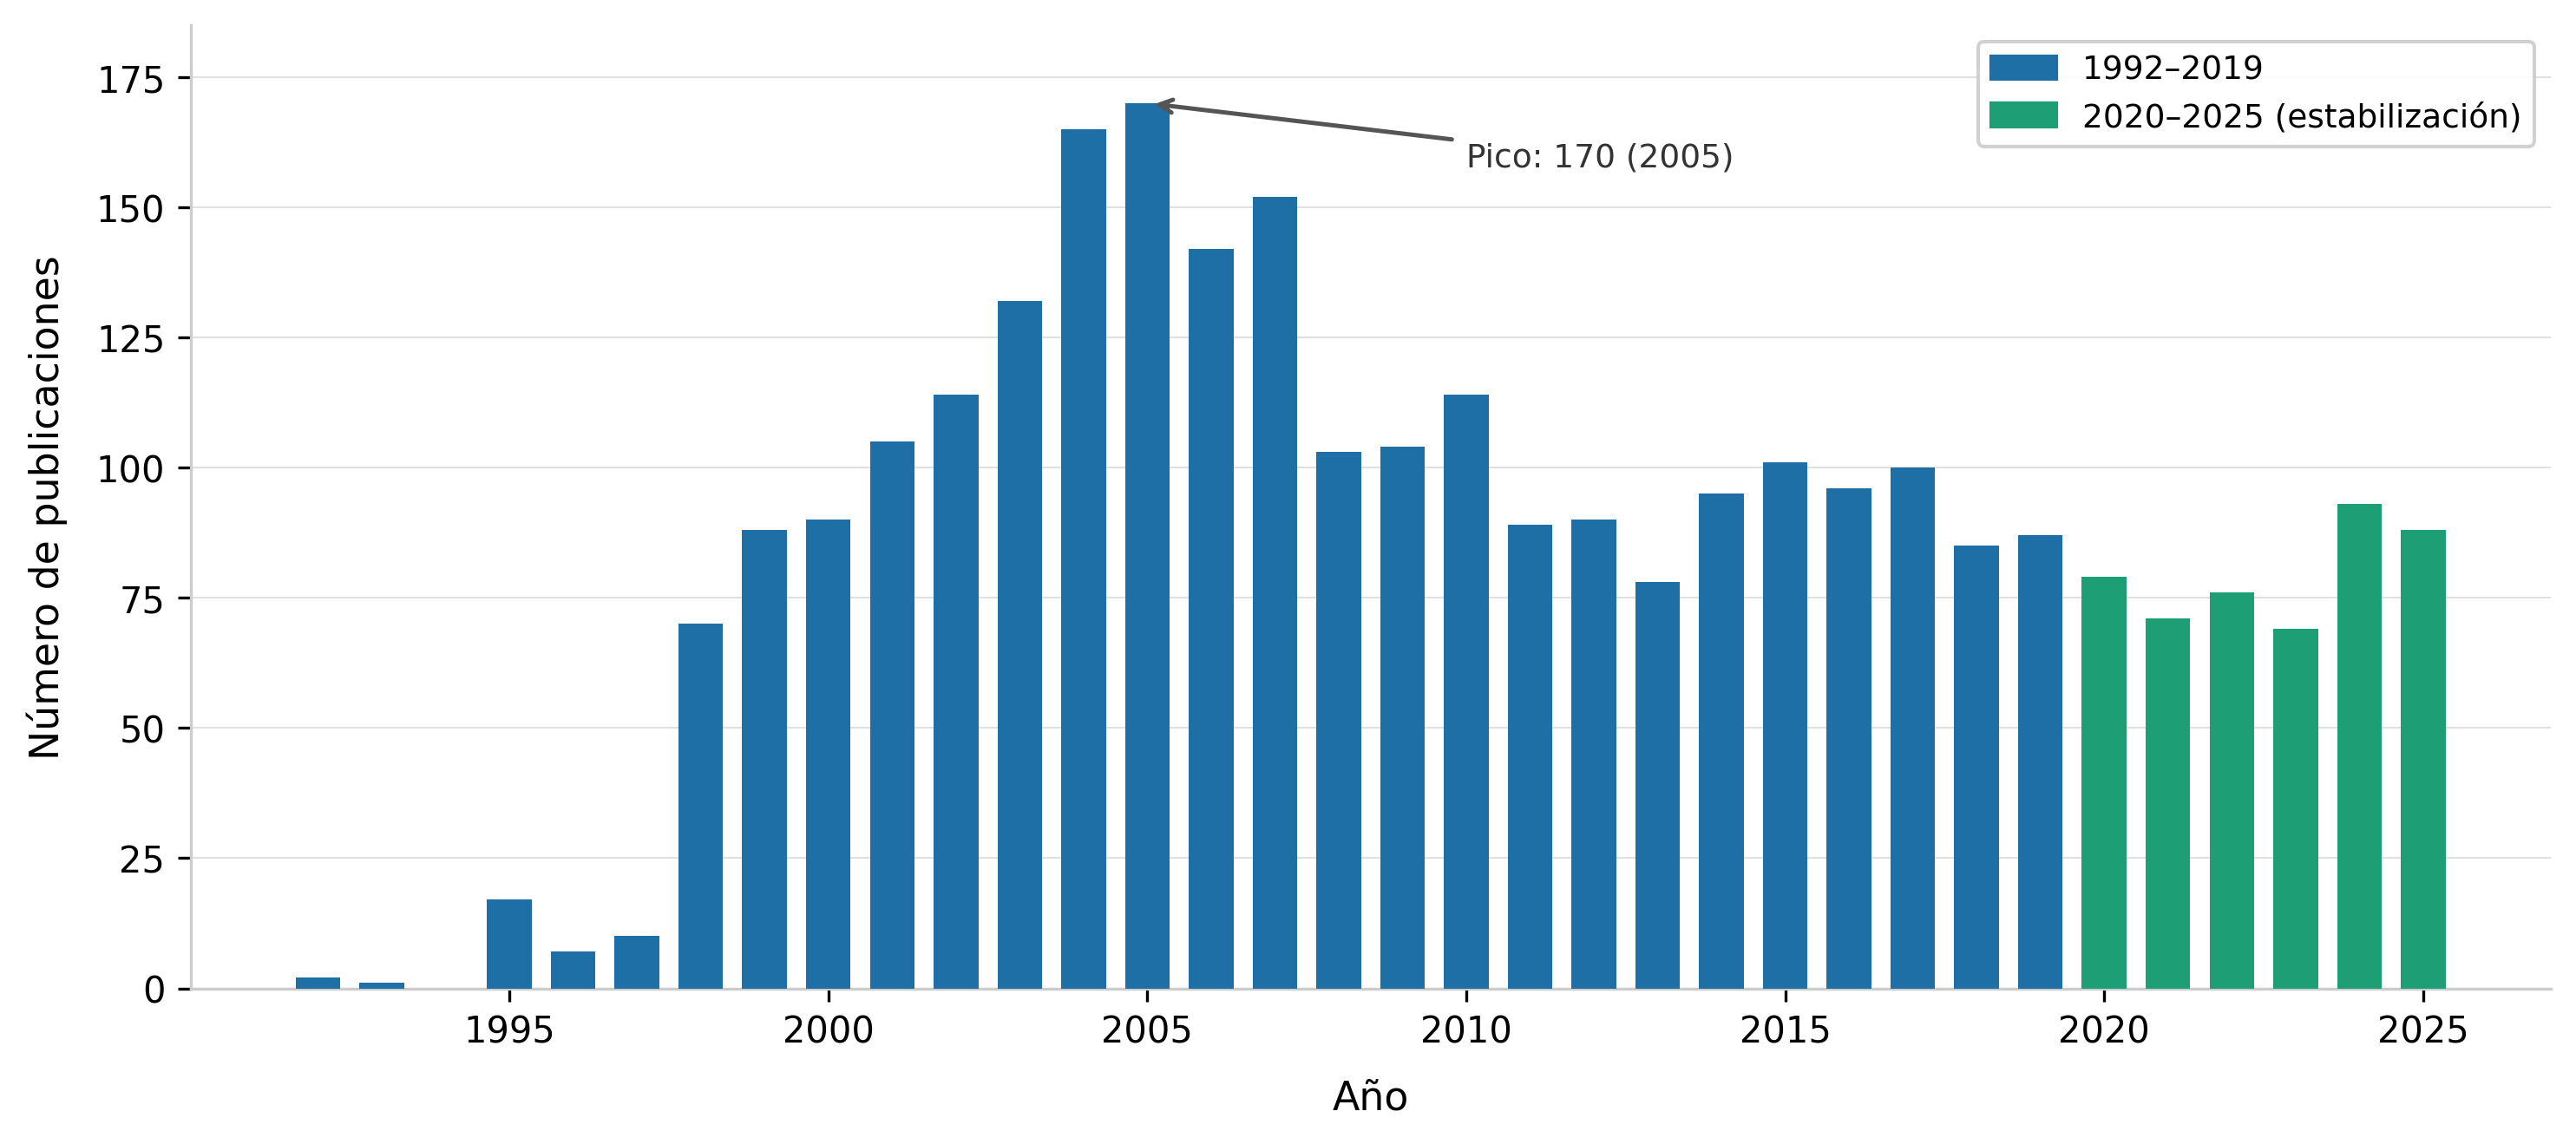
\includegraphics[width=0.92\textwidth]{figuras/tendencia_scopus.png}
  \caption{Tendencia de publicaciones sobre detección de \ac{MAP} en Scopus
           (palabras clave: \textit{landmine AND detection}). Se observa un
           pico máximo en 2004--2005 y una estabilización en torno a las
           80 publicaciones anuales en el período 2020--2025.}
  \label{fig:tendencia_scopus}

  {\footnotesize Fuente: elaboración propia con base en datos de Scopus.}
\end{figure}

Adicionalmente, de la revisión realizada por el grupo \ac{PSI}, un aspecto
diferenciador relevante es que ninguno de los trabajos con imágenes multiespectrales
o hiperespectrales identificados reporta experimentos con minas enterradas en
condiciones de siembra real prolongada ---es decir, con vegetación en crecimiento
libre durante semanas o meses sobre las zonas de mina---. El trabajo previo del
grupo \ac{PSI} con termografía infrarroja \cite{tenorio2024} sí opera en campo
real, pero explota la señal térmica aguda generada horas después del enterramiento,
no el estrés vegetal crónico acumulado. Este trabajo incluye esa condición de siembra prolongada, más representativa
del desminado humanitario real, donde las minas permanecen enterradas
por años.

De la revisión bibliográfica realizada es posible identificar cuatro métodos
predominantes de localización de \ac{MAP}: el \ac{GPR}, los \ac{MD}, las
cámaras infrarrojas y las cámaras multiespectrales. El \ac{GPR} emite pulsos
electromagnéticos que detectan cambios en las propiedades dieléctricas del
subsuelo, pero requiere operar muy cerca del terreno peligroso. Los \ac{MD}
son poco eficaces con minas de fabricación artesanal de contenido metálico
mínimo. Las cámaras infrarrojas y multiespectrales fundamentan su
funcionamiento en el procesamiento de imágenes capturadas en distintas
bandas del espectro, ofreciendo detección a distancia sin contacto con el
terreno \cite{barnawi2022}.

\subsection{Antecedentes internacionales}

A nivel internacional, el uso de imágenes multiespectrales e hiperespectrales
para la detección remota de \ac{MAP} ha ganado fuerza desde los años 90.

Un trabajo pionero es el de Clark \etal{} \cite{clark2000}, quienes
utilizaron una cámara Xybion de \textbf{seis bandas espectrales} (400--900~nm,
solo espectro visible) montada en un helicóptero para detectar minas
\textbf{metálicas, plásticas y sustitutos}, principalmente en superficie.
Su metodología extrae 54 características estadísticas (9 por banda) y selecciona
las más discriminativas mediante Sequential Forward Selection, utilizando una red
neuronal probabilística como clasificador. Con un conjunto de datos pequeño y en
condiciones de laboratorio, logró una Probabilidad de Detección (PD~=~1.0) ---
equivalente a una sensibilidad del 100\,\%--- y una Probabilidad de Falsa Alarma
(PFA~=~0.036) entrenando con minas metálicas y plásticas combinadas. Estos
resultados, aunque prometedores, fueron obtenidos en condiciones controladas sin
vegetación real, lo que limita su comparación directa con el presente trabajo.
Esta metodología de extracción de características estadísticas por banda es el
antecedente metodológico más directo del presente trabajo.

Makki \etal{} \cite{makki2017} presentaron una revisión sistemática de los
métodos de detección mediante imágenes hiperespectrales, demostrando que
la respuesta espectral de las minas con carcasa de plástico difiere de la
reflectancia del material de fondo, con tasas de detección reportadas en la
literatura superiores al 90\,\% en condiciones controladas. En su tesis doctoral
\cite{makki2017thesis}, el mismo autor desarrolló métodos de procesamiento
hiperespectral y reducción de dimensionalidad, señalando que la alta cantidad
de bandas de los sensores hiperespectrales requiere estrategias de selección
de características para ser operativos en campo --- motivación directa para el
uso de cámaras multiespectrales de pocas bandas seleccionadas.

Silva \etal{} \cite{silva2019} compararon clasificadores convencionales
contra una \ac{CNN} utilizando una cámara multiespectral Quest Condor3 de
\textbf{tres canales} (400--1000~nm) más una cámara térmica FLIR, en estructura
fija de laboratorio y campo exterior. Trabajaron con minas \textbf{antipersona
y antitanque plásticas} en suelo de arena (0--50~mm de profundidad), logrando
exactitud del 97\,\% en ambientes controlados. Evidenciaron que la profundidad
de enterramiento y las condiciones del entorno influyen significativamente en la
eficacia.
A diferencia de Silva \etal{}, aquí se trabaja con vegetación en crecimiento libre
y profundidades de hasta 70~mm en terreno de campo real.

Qiu \etal{} \cite{qiu2023} propusieron un sistema en \ac{UAV} con cámara
Sequoia de \textbf{cuatro bandas} (Verde, Rojo, Red Edge, NIR) y fusión YOLOv5,
logrando recall de 0.906 con RGB+NIR frente a 0.848 con RGB solo, demostrando la
ventaja de incorporar NIR. Vivoli \etal{} \cite{vivoli2024} implementaron detección
en tiempo real de minas superficiales con imágenes RGB y YOLO, superando el
90\,\% en campo real.

\subsection{Antecedentes nacionales}

En Colombia, la lucha contra las \ac{MAP} ha impulsado diversas
iniciativas de investigación centradas en técnicas de detección adaptadas
a las particularidades del conflicto y el terreno nacional.

Los trabajos más relevantes son los del grupo \ac{PSI}, que comparten el
mismo tipo de mina, terreno y condiciones de campo. Forero \etal{}
\cite{forero2022} lograron detectar \ac{MAP} tipo quiebrapatas con sensibilidad
del 97.1\,\% usando una cámara termográfica en \ac{UAV} a \SI{1}{m} y un
clasificador \ac{MLP}. Tenorio \etal{} \cite{tenorio2024} ampliaron el estudio
a alturas de 1--5~m, logrando exactitud del 92.13\,\% y sensibilidad del
82.4\,\% sobre 260 imágenes de prueba. A diferencia del enfoque térmico ---que
detecta contraste de temperatura agudo y depende del horario de captura---,
el enfoque multiespectral propuesto detecta perturbaciones crónicas del suelo y
la vegetación, con señal más estable temporalmente.

Cardona \etal{} \cite{cardona2014} revisaron tecnologías de detección en
Antioquia, identificando los \ac{MD}, el \ac{GPR} y las cámaras infrarrojas
y multiespectrales como las más viables para el contexto colombiano. Tovar
\cite{tovar2017} exploró la fusión de datos de múltiples sensores para
determinar la presencia de \ac{MAP} en una tesis de maestría de 2017;
aunque concluye que la combinación de sensores mejora la tasa de detección,
no reporta métricas numéricas comparables con los demás trabajos revisados,
no trabaja específicamente con imágenes multiespectrales, y sus condiciones
de experimentación no son equiparables a las del presente trabajo.

\subsection{Discusión de antecedentes}

La Tabla~\ref{tab:antecedentes} sintetiza los trabajos más relevantes,
cubriendo los aspectos metodológicos clave que permiten compararlos con el
presente trabajo.

\begin{table}[H]
\centering
\caption{Comparación de trabajos de referencia en detección de \ac{MAP}}
\label{tab:antecedentes}
\footnotesize
\begin{adjustbox}{width=1.15\textwidth,center}
\begin{tabular}{p{2.0cm}p{2.2cm}p{2.4cm}p{2.0cm}p{1.4cm}p{2.2cm}}
\toprule
\textbf{Trabajo} & \textbf{Sensor} & \textbf{Clasif.} &
\textbf{Métrica} & \textbf{Altura} & \textbf{Plataforma / entorno} \\
\midrule
Clark \etal{} \cite{clark2000}
  & MS 6 bandas & PNN & PD=1.0, PFA=0.036 & 76--137 m & Avión, exterior \\
Silva \etal{} \cite{silva2019}
  & MS 3 canales & SVM / CNN & OA 97\,\% & N/E & Estructura fija, lab./campo \\
Forero \etal{} \cite{forero2022}
  & Térmica IR & MLP & Sens. 97.1\,\% & 1 m & UAV, campo real \\
Tenorio \etal{} \cite{tenorio2024}
  & Térmica IR & MLP & Sens. 82.4\,\% & 1--5 m & UAV, campo real \\
Qiu \etal{} \cite{qiu2023}
  & MS 4 bandas & YOLOv5 & Recall 0.906 & N/E & UAV, campo real \\
Vivoli \etal{} \cite{vivoli2024}
  & Espectro visible & YOLO & Prec./Recall $>$90\,\% & N/E & UAV, tiempo real \\
\midrule
\textbf{Este trabajo}
  & \textbf{MS 5 bandas} & \textbf{EasyEns.~x10 XGBoost} & \textbf{AUC 0.947 / Sens. 82.3\,\%} & \textbf{1 m} & \textbf{Soporte estac., campo real} \\
\bottomrule
\multicolumn{6}{l}{\small MS: Multiespectral; estac.: sistema estacionario; N/E: no especificada.} \\
\multicolumn{6}{l}{\small OA: Overall Accuracy; Sens.: Sensibilidad; PD: Prob. Detección; PFA: Prob. Falsa Alarma.} \\
\multicolumn{6}{l}{\small AUC calculado con validación LOSO; Sens. con umbral fijo~=~0.5 (EasyEnsemble).} \\
\multicolumn{6}{l}{\small Los demás trabajos reportan métricas con partición aleatoria o conjunto de prueba fijo.}
\end{tabular}
\end{adjustbox}

  {\footnotesize Fuente: elaboración propia.}
\end{table}

Las Tablas~\ref{tab:comparacion_ms_features} y~\ref{tab:comparacion_ms_dataset}
profundizan la comparación exclusivamente entre los trabajos que emplean imágenes
multiespectrales, analizando aspectos técnicos directamente comparables con el
presente trabajo: el tipo y cantidad de características extraídas, el método de
selección y los parámetros del clasificador (Tabla~\ref{tab:comparacion_ms_features}),
así como el tamaño y balance del dataset, la estrategia de validación y las
condiciones de terreno y enterramiento (Tabla~\ref{tab:comparacion_ms_dataset}).
Esta comparación ubica los aportes metodológicos del presente trabajo
respecto al estado del arte multiespectral.

\clearpage
\begin{landscape}
\begin{table}
\centering
\caption{Comparación técnica (parte 1): características y clasificadores ---
         trabajos con imágenes multiespectrales para detección de \ac{MAP}}
\label{tab:comparacion_ms_features}
\footnotesize
\begin{tabularx}{\linewidth}{p{1.8cm} X X X p{2.5cm}}
\toprule
\textbf{Trabajo} & \textbf{Características extraídas} &
\textbf{Método de selección} & \textbf{Clasificador y parámetros clave} &
\textbf{Tamaño de ventana/ROI} \\
\midrule
Clark \etal{} \cite{clark2000}
  & 54 features: 9 estadísticas por banda (máx., mín., rango, media, std,
    asimetría, curtosis, energía, entropía) × 6 bandas
  & Sequential Forward Selection (SFS) con distancia de Bhattacharyya;
    se seleccionan 3 features finales
  & Red Neuronal Probabilística (PNN); parámetro $\sigma$ optimizado por
    tipo de mina; postprocesamiento por tamaño y forma
  & Tile 5×5 px por banda \\
\addlinespace
Silva \etal{} \cite{silva2019}
  & 264 features: estadísticas de orden superior + GLCM (textura:
    contraste, energía, correlación, homogeneidad a 0°, 45°, 90°, 135°)
    + índices espectrales
  & Algoritmo Relief (\textit{método de filtro}); features normalizadas
    al rango [0,\,1]
  & SVM kernel polinomial grado 8, algoritmo ISDA (\textit{Iterative Single Data Algorithm}, mejor exactitud);
    CNN con 3 capas conv. (filtros 64/128/256), batch norm., ReLU,
    pooling; hasta 200 épocas
  & ROI 10×10 px (AP); 80×80 px (AT) \\
\addlinespace
Qiu \etal{} \cite{qiu2023}
  & Mapas de características generados automáticamente por la CNN
    (no hay extracción manual de features)
  & Implícita en la arquitectura CNN (YOLOv5)
  & YOLOv5 \textit{end-to-end}; alturas de vuelo 3 y 8~m;
    solapamiento de imágenes 80\,\%
  & N/E (detección directa sobre imagen completa) \\
\addlinespace
\textbf{Este trabajo}
  & \textbf{378 features: 9 estadísticas (media, std, p25, p50, p75,
    mín., máx., mediana, rango) × 42 índices espectrales de
    vegetación, suelo y humedad (NDVI, NDRE, EVI, NDWI, BSI, SAVI\ldots)}
  & \textbf{Importancia de ganancia XGBoost (\textit{embedded}, undersampling 1:1 por fold);
    top-70 de 378; óptimo determinado por curva AUC/Sens vs.\ $k$}
  & \textbf{EasyEnsemble~x10 XGBoost (10 sub-clasificadores, ratio~1:1);
    RF y SVM~RBF evaluados como comparación base}
  & \textbf{Ventana 128×128 px; solapamiento 50\,\%} \\
\bottomrule
\multicolumn{5}{l}{\small SFS: Sequential Forward Selection; GLCM: Gray Level Co-occurrence Matrix;
Relief: filtro basado en distancias entre instancias.} \\
\multicolumn{5}{l}{\small PNN: red neuronal probabilística; CNN: red neuronal convolucional;
AP: antipersona; AT: antitanque; N/E: no especificado.}
\end{tabularx}

  {\footnotesize Fuente: elaboración propia.}
\end{table}
\end{landscape}
\clearpage


\clearpage
\begin{landscape}
\begin{table}
\centering
\caption{Comparación técnica (parte 2): dataset, validación y condiciones experimentales ---
         trabajos con imágenes multiespectrales para detección de \ac{MAP}}
\label{tab:comparacion_ms_dataset}
\footnotesize
\begin{tabularx}{\linewidth}{p{1.8cm}X X p{2.0cm} X}
\toprule
\textbf{Trabajo} & \textbf{Tamaño y balance del dataset} &
\textbf{Estrategia de validación} & \textbf{Métrica} &
\textbf{Condiciones de terreno y minas} \\
\midrule
Clark \etal{} \cite{clark2000}
  & $\sim$100 muestras mina, $\sim$200 fondo (balance 1:2);
    reconocido por los autores como dataset pequeño
  & Hold-one-out durante entrenamiento; conjunto de prueba
    fijo separado
  & PD=1.0 PFA=0.036
  & Campo militar real con pasto, arena y zonas despejadas;
    minas principalmente en superficie (pocas enterradas);
    mezcla de minas metálicas, plásticas y sustitutos;
    sin control de vegetación ni tiempo de enterramiento \\
\addlinespace
Silva \etal{} \cite{silva2019}
  & AP indoor: 10,262 ROIs; AP outdoor: 7,056 ROIs;
    \textbf{balanceado artificialmente}
  & Holdout 85\,\% entreno / 15\,\% prueba (partición aleatoria)
  & OA 97\,\% Sens. 98.5\,\%
  & Arena de laboratorio (cajones indoor) y academia militar
    (outdoor); profundidades AP $\leq$5~mm, AT $\leq$10~mm;
    objetos enterrados $<$30~min \textbf{(sin señal crónica
    acumulada)}; suelo perturbado no detectado por el sistema \\
\addlinespace
Qiu \etal{} \cite{qiu2023}
  & 789 pares de imágenes;
    minas en superficie o semisuperficiales
  & N/E
  & Recall 0.906
  & Pasto natural con vegetación variable; $\sim$60\,\% de las
    minas cubiertas por vegetación; minas en superficie
    (no enterradas); alturas de vuelo 3 y 8~m \\
\addlinespace
\textbf{Este trabajo}
  & \textbf{14,901 ventanas; 487 positivos / 14,414 negativos;
    desbalance real 30:1 (no balanceado artificialmente)}
  & \textbf{LOSO con 6 sesiones de campo --- sin fuga de datos
    entre sesiones; validación cruzada aleatoria descartada
    (AUC=0.999 inflado; véase Sección~\ref{sec:loso})}
  & \textbf{AUC 0.947 Sens. 82.3\,\% (umbral~=~0.5)}
  & \textbf{Campo real con vegetación limitada en crecimiento
    libre $\sim$6~meses; minas enterradas 1--7~cm;
    objetos de interferencia enterrados a la misma profundidad;
    señal crónica confirmada en bandas NIR} \\
\bottomrule
\multicolumn{5}{l}{\small OA: Overall Accuracy; Sens.: Sensibilidad con umbral fijo~=~0.5 (EasyEnsemble);
N/E: no especificado; AP: antipersona; AT: antitanque.} \\
\multicolumn{5}{l}{\small Las métricas de Silva et al. se obtuvieron con dataset balanceado artificialmente;
las de este trabajo con desbalance real y validación LOSO.}
\end{tabularx}

  {\footnotesize Fuente: elaboración propia.}
\end{table}
\end{landscape}
\clearpage
Los trabajos del grupo \ac{PSI} \cite{forero2022,tenorio2024} son el
referente más directo: mismo tipo de mina, mismo terreno experimental y
vegetación real. Este trabajo añade el análisis multiespectral a esa línea,
con una señal distinta
a la térmica.

Un aspecto diferenciador frente a los antecedentes revisados es la contribución
discriminativa de las bandas Red Edge y \ac{NIR}, observada con el etiquetado
preciso por bounding box ---aspecto poco explorado en los trabajos previos. Además, Clark~\etal{} y Silva~\etal{} operaron sin vegetación
real; este trabajo se realizó en campo con vegetación en crecimiento libre.

% -------------------------------------------------------------
\section{Mina Antipersona}

Las \ac{MAP} son artefactos explosivos diseñados para detonarse por la
presencia o proximidad de una persona, con el fin de incapacitarla,
herirla o matarla. Se activan típicamente al ser pisadas o al tensar un
cable trampa que libera una carga explosiva. En Colombia se ha identificado
gran variedad de minas, de las cuales más del 90\,\% son de fabricación
artesanal \cite{ocha2015,unicef2021}.

\subsection{Tipos de minas antipersona más comunes en Colombia}

La mayoría de \ac{MAP} colombianas son de fabricación artesanal e
improvisada, con mínimos componentes metálicos, fabricadas con materiales
de fácil acceso como madera, tubos de \ac{PVC}, plásticos, fragmentos de
metal, vidrios y explosivos caseros \cite{mineban2010,gutierrez2014}:

\textbf{Mina quiebrapatas.} La más común y la que más víctimas cobra \cite{hernandez2023}.
Diseñada para explotar cuando es pisada, fabricada con tubo de \ac{PVC},
alambre, batería de 1.5~V, explosivo (dinamita o nitrato de amonio) y
fragmentos de metal. Es el tipo de mina emulada en el presente trabajo.

\textbf{Mina tipo sombrero chino.} Rango efectivo de \SI{25}{m}.
Fabricada con explosivo casero R-1 y trozos de metal, con sistema de
activación eléctrico mediante cable conductor de 200 a 300~m.

\textbf{Mina tipo cajón.} Elaborada con caja de madera y dinamita o
explosivo casero R-1. Utilizada principalmente contra vehículos.

La predominancia de materiales no metálicos es la razón por la cual los
detectores de metales convencionales son ineficaces para la mayoría de las
\ac{MAP} colombianas, justificando la búsqueda de métodos de detección
alternativos basados en propiedades ópticas y espectrales.

% -------------------------------------------------------------
\section{Tipos de suelos}

El territorio colombiano comprende una amplia variedad de suelos determinados
por su diversidad geográfica y climática. En las zonas de alta presencia de
\ac{MAP} predominan suelos arcillosos y franco-arcillosos, suelos con alto
contenido orgánico en áreas selváticas tropicales y suelos arenosos
\cite{IsaacAnteproyecto}.

Este trabajo se enfoca en suelos con textura arenosa y vegetación limitada,
condición del terreno experimental utilizado en el campus de la Universidad
del Valle, sede Meléndez --- el mismo terreno empleado en los trabajos previos
del grupo \ac{PSI} \cite{forero2022,tenorio2024}. El contraste espectral
entre el suelo perturbado (sobre la mina) y el suelo sin alteración es más
pronunciado en suelos de textura gruesa, donde la remoción del material
durante el enterramiento genera cambios de color y textura superficial más
evidentes que en suelos arcillosos compactos \cite{nanni2006}.

% -------------------------------------------------------------
\section{Imágenes multiespectrales}

A diferencia de una cámara convencional RGB, un sensor multiespectral
captura información en múltiples bandas del espectro electromagnético.
La cámara produce varias imágenes de la misma escena, cada una
correspondiente a una banda específica de longitudes de onda; al
superponer o analizar conjuntamente las bandas, es posible distinguir
objetos o características que pasan desapercibidas al analizar únicamente el espectro visible
\cite{navarro2024}.

\subsection{La cámara MicaSense RedEdge-MX}

Para este trabajo se empleó la cámara MicaSense RedEdge-MX, que captura
imágenes en cinco bandas espectrales con resolución de 1.2~Mpx por banda.
Las características de cada banda se resumen en la
Tabla~\ref{tab:bandas_micasense}.

\begin{table}[H]
\centering
\caption{Especificaciones de las bandas de la cámara MicaSense RedEdge-MX}
\label{tab:bandas_micasense}
\begin{tabular}{clcc}
\toprule
\textbf{Banda} & \textbf{Nombre} & \textbf{Centro (\si{nm})} &
\textbf{Ancho FWHM (\si{nm})} \\
\midrule
1 & Azul (Blue)              & 475 & 32 \\
2 & Verde (Green)            & 560 & 27 \\
3 & Rojo (Red)               & 668 & 16 \\
4 & Red Edge                 & 717 & 12 \\
5 & Infrarrojo Cercano (NIR) & 842 & 57 \\
\bottomrule
\end{tabular}

  {\footnotesize Fuente: elaboración propia.}
\end{table}

La cámara dispone de cinco objetivos físicamente separados, uno por banda,
lo que implica que las imágenes de cada banda requieren un proceso de
corrección geométrica (Sección~\ref{sec:alineacion}).

\subsection{Firma espectral y mecanismos de detección de MAP}

Los distintos materiales reflejan o emiten radiación de manera diferente
en cada banda espectral; a esto se denomina \textit{firma espectral}.
En el caso de una \ac{MAP} enterrada, la anomalía espectral puede
manifestarse de tres formas principales \cite{qiu2023,barnawi2022}:

\textbf{Perturbación del color superficial del suelo.} El proceso de
enterramiento remueve y redeposita el material del suelo, alterando su
composición superficial. El suelo subsuperficial expuesto tiene una
composición mineralógica y un contenido de materia orgánica diferente al
suelo superficial original, generando diferencias de color detectables en
las bandas del espectro visible (Azul, Verde, Rojo). Este mecanismo opera
desde el momento del enterramiento y produce señales espectrales en índices
como \ac{VARI}, \ac{NDRB} y el ratio Rojo/Azul.

\textbf{Estrés vegetal diferencial — señal en Red Edge y NIR.}
Las plantas sobre una \ac{MAP} enterrada pueden responder al estrés mecánico
(compactación del suelo) y químico del material explosivo, generando cambios
en su contenido de clorofila y en la estructura del mesófilo foliar. La
clorofila absorbe fuertemente en las bandas roja y azul, y refleja en la
banda verde; cuando el contenido de clorofila disminuye por estrés, la
reflectancia en la banda \textbf{Red Edge} (\SI{717}{nm}) aumenta de forma
característica antes de que el estrés sea visible a simple vista
\cite{qiu2023}. La banda \textbf{\ac{NIR}} (\SI{842}{nm}) es sensible a la
estructura interna de la hoja (mesófilo): el estrés hídrico y mecánico
reduce la reflectancia \ac{NIR} al afectar los espacios de aire intercelulares
que generan la alta reflectancia infrarroja de la vegetación sana. Índices
que combinan estas bandas —\ac{NDRE}, \ac{NDVI}, y ratios NIR/Red— son
los más sensibles para detectar este tipo de estrés crónico. Este mecanismo
es de naturaleza acumulativa y se intensifica semanas o meses después del
enterramiento.

\textbf{Contraste térmico.} Las minas tienen propiedades térmicas distintas
al suelo, generando diferencias de temperatura detectables en imágenes
infrarrojas térmicas \cite{forero2022,tenorio2024}. Su señal es aguda y
transitoria, complementaria a los mecanismos espectrales.

\textbf{Implicación metodológica.} La precisión del etiquetado del
groundtruth determina cuál de estos mecanismos captura preferentemente el
clasificador. Un etiquetado grueso (toda la zona como positiva) tiende a privilegiar la
perturbación del color del suelo ---señal visible y distribuida en toda el área---,
mientras que un etiquetado ajustado por bounding box preserva mejor la señal
localizada de Red Edge y \ac{NIR}. El análisis de importancia del
Capítulo~\ref{cap:resultados} es \emph{consistente} con esta hipótesis: esas bandas
figuran entre las características relevantes del modelo.

% -------------------------------------------------------------
\section{Índices espectrales}
\label{sec:indices_espectrales}

Los índices espectrales son combinaciones matemáticas de dos o más bandas
diseñadas para resaltar características específicas de la superficie.
Los índices calculados en este trabajo se describen a continuación.

\subsection{Índices de vegetación}

El \ac{NDVI} es el índice de vegetación más ampliamente utilizado en
teledetección \cite{makki2017}:
\begin{equation}
  \text{NDVI} = \frac{\rho_{\text{NIR}} - \rho_{\text{Red}}}
                     {\rho_{\text{NIR}} + \rho_{\text{Red}}}
  \label{eq:ndvi}
\end{equation}
Sus valores van de $-1$ a $+1$; por encima de 0.5 se asocia a vegetación
densa y sana, por debajo de 0.2 a suelo desnudo o agua.

El \ac{NDRE} es análogo al \ac{NDVI} pero utiliza la banda Red Edge
(\SI{717}{nm}) en lugar de la banda Roja. La región Red Edge corresponde
al borde de absorción de la clorofila, donde la reflectancia transiciona
abruptamente de baja (rojo, absorbido por clorofila) a alta (NIR, reflejado
por estructura celular). Cambios en el contenido de clorofila desplazan
este borde, haciendo al \ac{NDRE} más sensible que el \ac{NDVI} a estrés
vegetal temprano — cuando el estrés aún no es visible a simple vista
\cite{makki2017}:
\begin{equation}
  \text{NDRE} = \frac{\rho_{\text{NIR}} - \rho_{\text{RedEdge}}}
                     {\rho_{\text{NIR}} + \rho_{\text{RedEdge}}}
  \label{eq:ndre}
\end{equation}

La banda \ac{NIR} (\SI{842}{nm}) es particularmente sensible a la estructura
interna de la hoja: la alta reflectancia infrarroja de la vegetación sana
proviene de los espacios de aire entre células del mesófilo, que actúan como
dispersores de radiación. El estrés hídrico y mecánico colapsa estos espacios,
reduciendo la reflectancia \ac{NIR}. Por esta razón, índices que involucran
\ac{NIR} —como \ac{NDVI}, \ac{NDRE} y el ratio NIR/Red— son los más
discriminativos para detectar estrés vegetal crónico inducido por el
enterramiento de \ac{MAP}.

El \ac{EVI} reduce el efecto del suelo de fondo y la saturación
atmosférica en zonas de alta densidad vegetal:
\begin{equation}
  \text{EVI} = 2.5 \cdot
  \frac{\rho_{\text{NIR}} - \rho_{\text{Red}}}
       {\rho_{\text{NIR}} + 6\,\rho_{\text{Red}} - 7.5\,\rho_{\text{Blue}} + 1}
  \label{eq:evi}
\end{equation}

El \ac{VARI} estima la fracción de cobertura vegetal usando exclusivamente
bandas visibles, siendo robusto ante variaciones de irradiancia. Es el
índice más discriminativo identificado en este trabajo:
\begin{equation}
  \text{VARI} = \frac{\rho_{\text{Green}} - \rho_{\text{Red}}}
                     {\rho_{\text{Green}} + \rho_{\text{Red}} - \rho_{\text{Blue}}}
  \label{eq:vari}
\end{equation}

\subsection{Índices de ratio entre bandas visibles}

El \ac{NDRB} cuantifica la diferencia normalizada entre las bandas roja
y azul, sensible a cambios en el color superficial del suelo:
\begin{equation}
  \text{NDRB} = \frac{\rho_{\text{Red}} - \rho_{\text{Blue}}}
                     {\rho_{\text{Red}} + \rho_{\text{Blue}}}
  \label{eq:ndrb}
\end{equation}

El \ac{NDGB} compara las bandas verde y azul, sensible a cambios en la
composición superficial del suelo:
\begin{equation}
  \text{NDGB} = \frac{\rho_{\text{Green}} - \rho_{\text{Blue}}}
                     {\rho_{\text{Green}} + \rho_{\text{Blue}}}
  \label{eq:ndgb}
\end{equation}

El ratio Rojo/Azul es un indicador directo del color del suelo; suelos con
mayor contenido de óxidos de hierro o materia orgánica alterada presentan
valores más altos:
\begin{equation}
  \text{Red/Blue} = \frac{\rho_{\text{Red}}}{\rho_{\text{Blue}}}
  \label{eq:redblue}
\end{equation}

\subsection{Índices de suelo y textura}

El \ac{BSI} resalta áreas de suelo desnudo combinando múltiples bandas:
\begin{equation}
  \text{BSI} = \frac{(\rho_{\text{Red}} + \rho_{\text{Blue}}) -
                     (\rho_{\text{NIR}} + \rho_{\text{Green}})}
                    {(\rho_{\text{Red}} + \rho_{\text{Blue}}) +
                     (\rho_{\text{NIR}} + \rho_{\text{Green}})}
  \label{eq:bsi}
\end{equation}

El \ac{HI} cuantifica el tono de color del suelo en el espacio visible,
siendo sensible a cambios en la mineralogía superficial y el contenido de
materia orgánica:
\begin{equation}
  \text{HI} = \frac{2\,\rho_{\text{Red}} - \rho_{\text{Green}} - \rho_{\text{Blue}}}
                   {2(\rho_{\text{Red}} - \rho_{\text{Blue}})}
  \label{eq:hi}
\end{equation}

El \textbf{NDSI} (\textit{Normalized Difference Soil Index}) cuantifica la
proporción entre la reflectancia roja y el infrarrojo cercano, siendo
sensible a la exposición de suelo desnudo y a perturbaciones superficiales:
\begin{equation}
  \text{NDSI} = \frac{\rho_{\text{Red}} - \rho_{\text{NIR}}}
                     {\rho_{\text{Red}} + \rho_{\text{NIR}}}
  \label{eq:ndsi}
\end{equation}

% -------------------------------------------------------------
\section{Calibración radiométrica}
\label{sec:calibracion_teorica}

La calibración radiométrica transforma los valores de nivel digital~(DN)
capturados por el sensor en valores de reflectancia de superficie,
independientes de las condiciones de iluminación. Sin calibración, los
valores de DN varían entre sesiones según la hora del día, la nubosidad
y el ángulo solar, impidiendo comparar imágenes de distintos momentos.

El método empleado utiliza un \ac{CRP}, que es un panel de material
difusamente reflectante con valores de reflectancia nominal conocidos y
certificados para cada banda espectral: Blue~=~0.490, Green~=~0.491,
Red~=~0.491, Red Edge~=~0.488 y NIR~=~0.490. Estos valores, proporcionados
por el fabricante, establecen la relación lineal entre el nivel digital
(DN) capturado por el sensor y la reflectancia de superficie real:
\begin{equation}
  \rho_{\text{sup}}(\lambda) =
  \frac{\text{DN}_{\text{zona}}(\lambda)}{\text{DN}_{\text{panel}}(\lambda)}
  \cdot \rho_{\text{panel}}(\lambda)
  \label{eq:calibracion}
\end{equation}
\noindent donde $\rho_{\text{panel}}(\lambda)$ es la reflectancia nominal
del panel para la banda $\lambda$.

% -------------------------------------------------------------
\section{Alineación de bandas}
\label{sec:alineacion}

Dado que la MicaSense RedEdge-MX contiene cinco objetivos físicamente
separados, las bandas no están perfectamente alineadas entre sí. A
\SI{1}{m} de altura, el paralaje entre lentes genera un desalineamiento
residual que debe corregirse para que los índices espectrales calculados
a nivel de píxel sean representativos.

La corrección geométrica entre bandas se realiza mediante \ac{SIFT}
\cite{sift_lowe2004}, algoritmo seleccionado por tres razones frente a
otras alternativas como ORB, SURF o correlación cruzada:
(1)~es invariante a cambios de escala,
rotación e iluminación entre bandas, condición importante dado que los
cinco lentes de la MicaSense capturan con ligeras diferencias de perspectiva
y exposición; (2)~produce descriptores robustos que funcionan bien en
texturas naturales como suelo y vegetación, a diferencia de métodos basados
en bordes (Harris, FAST) que requieren contornos bien definidos; y
(3)~permite estimar una homografía global mediante RANSAC, que corrige el
desplazamiento promedio entre bandas de forma eficiente con el conjunto de
datos disponible. Como alternativa cuando \ac{SIFT} no converge se utiliza
el algoritmo ECC (\textit{Enhanced Correlation Coefficient}), que opera por
optimización iterativa y es más robusto en imágenes con poco contraste.

A \SI{1}{m} de captura el paralaje entre los cinco lentes es
significativamente mayor que a distancias típicas de vuelo. La homografía
global corrige el desplazamiento promedio pero no puede compensar el
paralaje local generado por objetos tridimensionales como la vegetación.
Este efecto es inherente a la captura en campo cercano y es aceptable para
la extracción de características estadísticas por ventana.

% -------------------------------------------------------------
\section{Selección de características en teledetección}

En los trabajos de detección de \ac{MAP} con imágenes multiespectrales,
las características más empleadas son de naturaleza estadística y espectral.
Clark \etal{} \cite{clark2000} extrajeron estadísticas por banda (máximo,
media, curtosis, energía y desviación estándar) sobre regiones de interés,
seleccionando las más discriminativas mediante Sequential Forward Selection.
Silva \etal{} \cite{silva2019} utilizaron características de textura
derivadas de matrices de co-ocurrencia (GLCM) combinadas con índices
espectrales. Qiu \etal{} \cite{qiu2023} emplearon mapas de características
generados por redes convolucionales sobre composiciones multibanda. En el
presente trabajo se extraen estadísticas descriptivas (media,
desviación estándar, percentiles) sobre más de 40 índices espectrales de
vegetación, suelo y humedad calculados a partir de las cinco bandas de la
MicaSense RedEdge-MX, generando 378 características por ventana.

La selección de características es el proceso de identificar el subconjunto
mínimo de variables que preserva el poder predictivo del modelo completo.
En teledetección con datos de alta dimensionalidad cumple tres funciones:
reduce el sobreajuste al eliminar variables ruidosas o redundantes, mejora
la interpretabilidad del modelo identificando qué índices espectrales son
físicamente relevantes, y reduce el costo computacional de la clasificación.
Los métodos de selección de características se agrupan en tres familias
\cite{makki2017,silva2019}:

\begin{itemize}
  \item \textbf{Métodos de filtro:} evalúan cada característica de forma
    independiente mediante una métrica estadística (correlación, información
    mutua, Fisher Discriminant Ratio) y seleccionan las mejor puntuadas, sin
    intervención del clasificador. Son rápidos pero no capturan interacciones
    entre características.
  \item \textbf{Métodos envolventes (\textit{wrapper}):} utilizan el propio
    clasificador para evaluar subconjuntos de características por búsqueda
    exhaustiva o heurística (hacia adelante, hacia atrás). Son más precisos
    pero computacionalmente costosos.
  \item \textbf{Métodos embebidos:} la selección ocurre durante el
    entrenamiento del clasificador. El \ac{RF} pertenece a esta categoría:
    calcula la importancia de cada característica como la reducción media de
    impureza de Gini aportada a lo largo de todos los árboles del bosque
    \cite{breiman2001}.
\end{itemize}

En este trabajo se utiliza el método embebido de importancia por ganancia
de \ac{XGBoost} (reducción acumulada del error al dividir por cada
característica). La selección se realiza dentro del mismo clasificador final
(EasyEnsemble x10 XGBoost) y por cada fold de validación, con submuestreo
1:1, garantizando coherencia metodológica entre selección y clasificación.
Se seleccionan las 70 características de mayor importancia (\textit{top-70}).
A diferencia de Clark \etal{}, que aplicaron selección de características
sobre estadísticas de banda con un clasificador de red neuronal probabilística,
el presente trabajo combina el etiquetado preciso por bounding box con la
selección embebida de XGBoost; el análisis de importancia resultante es consistente
con una contribución discriminativa de las bandas Red Edge y \ac{NIR} ---aspecto
poco explorado en los trabajos revisados.

% -------------------------------------------------------------
\section{Algoritmos de clasificación}

La detección de \ac{MAP} se formula como un problema de clasificación
binaria supervisada: cada ventana se clasifica como \textit{con MAP} o
\textit{sin MAP}. A continuación se describen los algoritmos seleccionados
con base en su desempeño reportado en la literatura de teledetección y
detección de \ac{MAP} \cite{silva2019, barnawi2022, chen2016}.

\subsection{Bosque aleatorio (Random Forest)}

El \ac{RF} construye múltiples árboles de decisión durante el entrenamiento
y combina sus predicciones por votación mayoritaria \cite{breiman2001}.
Cada árbol se entrena sobre una muestra con reemplazo (\textit{bagging}),
y en cada nodo se selecciona aleatoriamente un subconjunto de
características, reduciendo la correlación entre árboles y mejorando la
generalización.

El \ac{RF} es el clasificador estándar en teledetección con bases de datos de
tamaño moderado \cite{silva2019} --- típicamente entre 1\,000 y 100\,000
muestras ---, rango que incluye la base de datos de este trabajo
(14\,901 ventanas). Sus propiedades son especialmente relevantes para este
problema: es invariante a la escala (no requiere normalización), robusto
con alta dimensionalidad (378 características), produce importancia de
características con valor interpretativo, y ofrece mecanismos para tratar
el desbalance de clases. A diferencia de
las redes neuronales profundas, generaliza bien con pocos miles de muestras
sin requerir grandes cantidades de datos de entrenamiento.

\subsection{Máquina de Vectores de Soporte (SVM)}

La \ac{SVM} busca el hiperplano de separación de máximo margen en el espacio
de características \cite{vapnik1995}. El núcleo RBF transforma implícitamente
el espacio a alta dimensión cuando los datos no son linealmente separables,
propiedad relevante para las 378 características espectrales del presente
trabajo. La \ac{SVM} requiere escalado previo; se aplica \texttt{StandardScaler}
ajustado dentro de cada pliegue \ac{LOSO} para evitar fuga de datos.

\subsection{XGBoost}

XGBoost (\textit{Extreme Gradient Boosting}) es un método de ensamble
basado en \textit{boosting}: construye árboles de decisión de forma
secuencial, donde cada árbol corrige los errores del anterior mediante
el gradiente de la función de pérdida \cite{chen2016}. A diferencia del \ac{RF} (árboles independientes por bagging), XGBoost
construye cada árbol corrigiendo los errores del anterior, lo que le
permite ajustarse a patrones más difíciles. En datos tabulares de alta
dimensionalidad, XGBoost supera al \ac{RF} cuando el volumen de datos es
suficiente \cite{qiu2023}. En este problema, las relaciones entre los índices
espectrales y la presencia de mina son altamente no lineales, lo que favorece a
XGBoost.

% -------------------------------------------------------------
\section{Estrategia de validación: Leave-One-Session-Out}
\label{sec:loso_teoria}

La estrategia de validación define cómo se reparten los datos entre
entrenamiento y prueba. Con partición aleatoria, ventanas de la misma imagen
pueden quedar en entrenamiento y prueba al mismo tiempo, inflando las
métricas ---en esta base de datos el AUC sube a 0.999 con partición
aleatoria frente a 0.947 con \ac{LOSO}---. En teledetección con sesiones
de campo, las condiciones ambientales de cada sesión correlacionan todas
las muestras de esa adquisición, haciendo el problema de fuga aún más
severo.

La estrategia \ac{LOSO} resuelve esto reservando en cada pliegue una sesión
de campo completa como conjunto de prueba y entrenando con las sesiones
restantes. Con $N$ sesiones se obtienen $N$ pliegues independientes, cada
uno evaluando la capacidad del modelo de generalizar a condiciones de
captura no vistas. Las métricas reportadas son el promedio de los $N$
pliegues. Esta estrategia es la recomendada en trabajos de detección
multiespectral donde la variabilidad entre sesiones de campo es la principal
fuente de incertidumbre \cite{silva2019}. Los detalles de implementación
para el presente trabajo se describen en la Sección~\ref{sec:loso}.